\section{Synchronization Algorithm}
\label{sec:sync_algo}
\subsection{Outline}
The ultimate objective of synchronized recording is to assign
the identical timestamp $T_n$ to all camera frames that are triggered
by the $n$-th synchronization pulse. This global time $T_n$ should
advance at a near constant rate with low jitter, and should on average correspond to the
time at which the frames arrive at the host.

When sync pulse number $n$ triggers a frame, two different sources of
timing information become available:
\begin{enumerate}
\item
The image time stamp $\etime{n}$ embedded with the image from camera
$i$. While the corresponding set of time stamps $\etime{}$ has low jitter,
it is generated by the camera, and can 
therefore not be directly compared to the host clock. Moreover, $\etime{}$
may drift over time from $\ejtime{}$, since the camera clocks are not disciplined. For
this reason we use the embedded timestamps only
for detecting dropped frames. For that purpose however, they are
indispensible.
\item
The time $\atime{n}$ when the frame from camera $i$ arrives at the
application layer. Although the set of arrival times $\atime{}$ is plagued
by large noise (cf Fig. \ref{fig:perioddist}), $\atime{}$ is consistently
measured by the host clock across all cameras. To be precise,
$\atime{n}$ is the time of arrival of frame $n$ from camera $i$,
{\em minus the current shutter time of camera $i$}. Subtracting off the
shutter time removes the systematic bias due to the fact that cameras
with longer shutter time settings will send their images later. So
although we will subsequently refer to $\atime{}$ as the arrival time,
it really is the arrival time {\em net of shutter time}.
\end{enumerate}

With these preliminary definitions, we can outline our strategy, which
consists of three steps:
\begin{itemize}
\item First, we establishes a low jitter estimate of the strobe period
  $\dt$. The strobe period is an estimate of the true time (as measured
  measured by the host clock) that elapses between sync pulses
  triggering the cameras.
\item With known strobe period, we maintain a per-camera clock
  $\ttime{}$ that upon
  frame arrival is advanced by the strobe period. The per-camera clock
  will thus inherit the low jitter property from the strobe
  period. While the arrival times $\atime{}$ may temporarily deviate
  from the corresponding times $\ttime{}$, on the long run and on average, $\ttime{}$ and
  $\atime{}$ agree. This is mainly due to the fact that $\ttime{}$ is updated with the ``true''
  strobe period $\dt$. An additional small correction term is added to
  the camera clock update to remove possible   drift.
\item Once a low-jitter per-camera clock is available, simple time
  proximity can be used to determine if a newly arriving frame
  can be associated with ones that have already been received, or
  if it is the first frame corresponding to the next sync pulse.
\end{itemize}

Fig. \ref{fig:arrival_vs_frame} shows the dramatic reduction of jitter
when going from raw arrival times $\atime{}$, shown as filled circles,
to the filtered camera times $\ttime{}$,
shown as crosses. The following subsections will describe in detail
how the filtering works.

\subsection{Estimating the strobe period}
Based on the frequency $f$ to which the pulse
generator is set, an initial estimate of the strobe period can be computed as
$\dt_0 = 1/f$. This serves as a starting point for an 
exponential moving average, which is updated whenever a new camera strobe period $\dta{n}$
becomes available for any camera $i$:
\begin{equation}
\label{eq:expavg}
\dtn{n} = (1-\alpha) \dtn{n-1}  + \alpha\ \dta{n}\ .
\end{equation}
Because of the possiblity of frame drops, the camera strobe period
$\dta{n}$ cannot simply be determined by subtracting $\atime{n-1}$
from $\atime{n}$. Rather, we first use the embedded image timestamps $\etime{}$
to find the number of frames that have passed:
\begin{equation}
\label{eq:nframes}
 k = \mathrm{round}((\etime{n} - \etime{\mathrm{prev}})/\dtn{n})\ .
\end{equation}

Then the strobe period for a camera is simply the time difference
of arrival times between two frames, divided by the number of frames:
\begin{equation*}
\dta{n} =  \frac{\atime{n} - \atime{n-k}}{k}\ .
\end{equation*}

The coefficient $\alpha$ in Eq. \ref{eq:expavg} is set such
as to average over a time horizon that is longer than any temporary
latency fluctuations, for instance $\tau=10$ seconds:
\begin{equation}
\alpha = 1/(f N \tau)\ .
\end{equation}

Fig. \ref{fig:expavg} shows the estimated $\dt$ as a function of
time. Notice how during the first few seconds the estimate is not well
established. During this warmup period, no frames are published.

\begin{figure}[h]
	\centering
	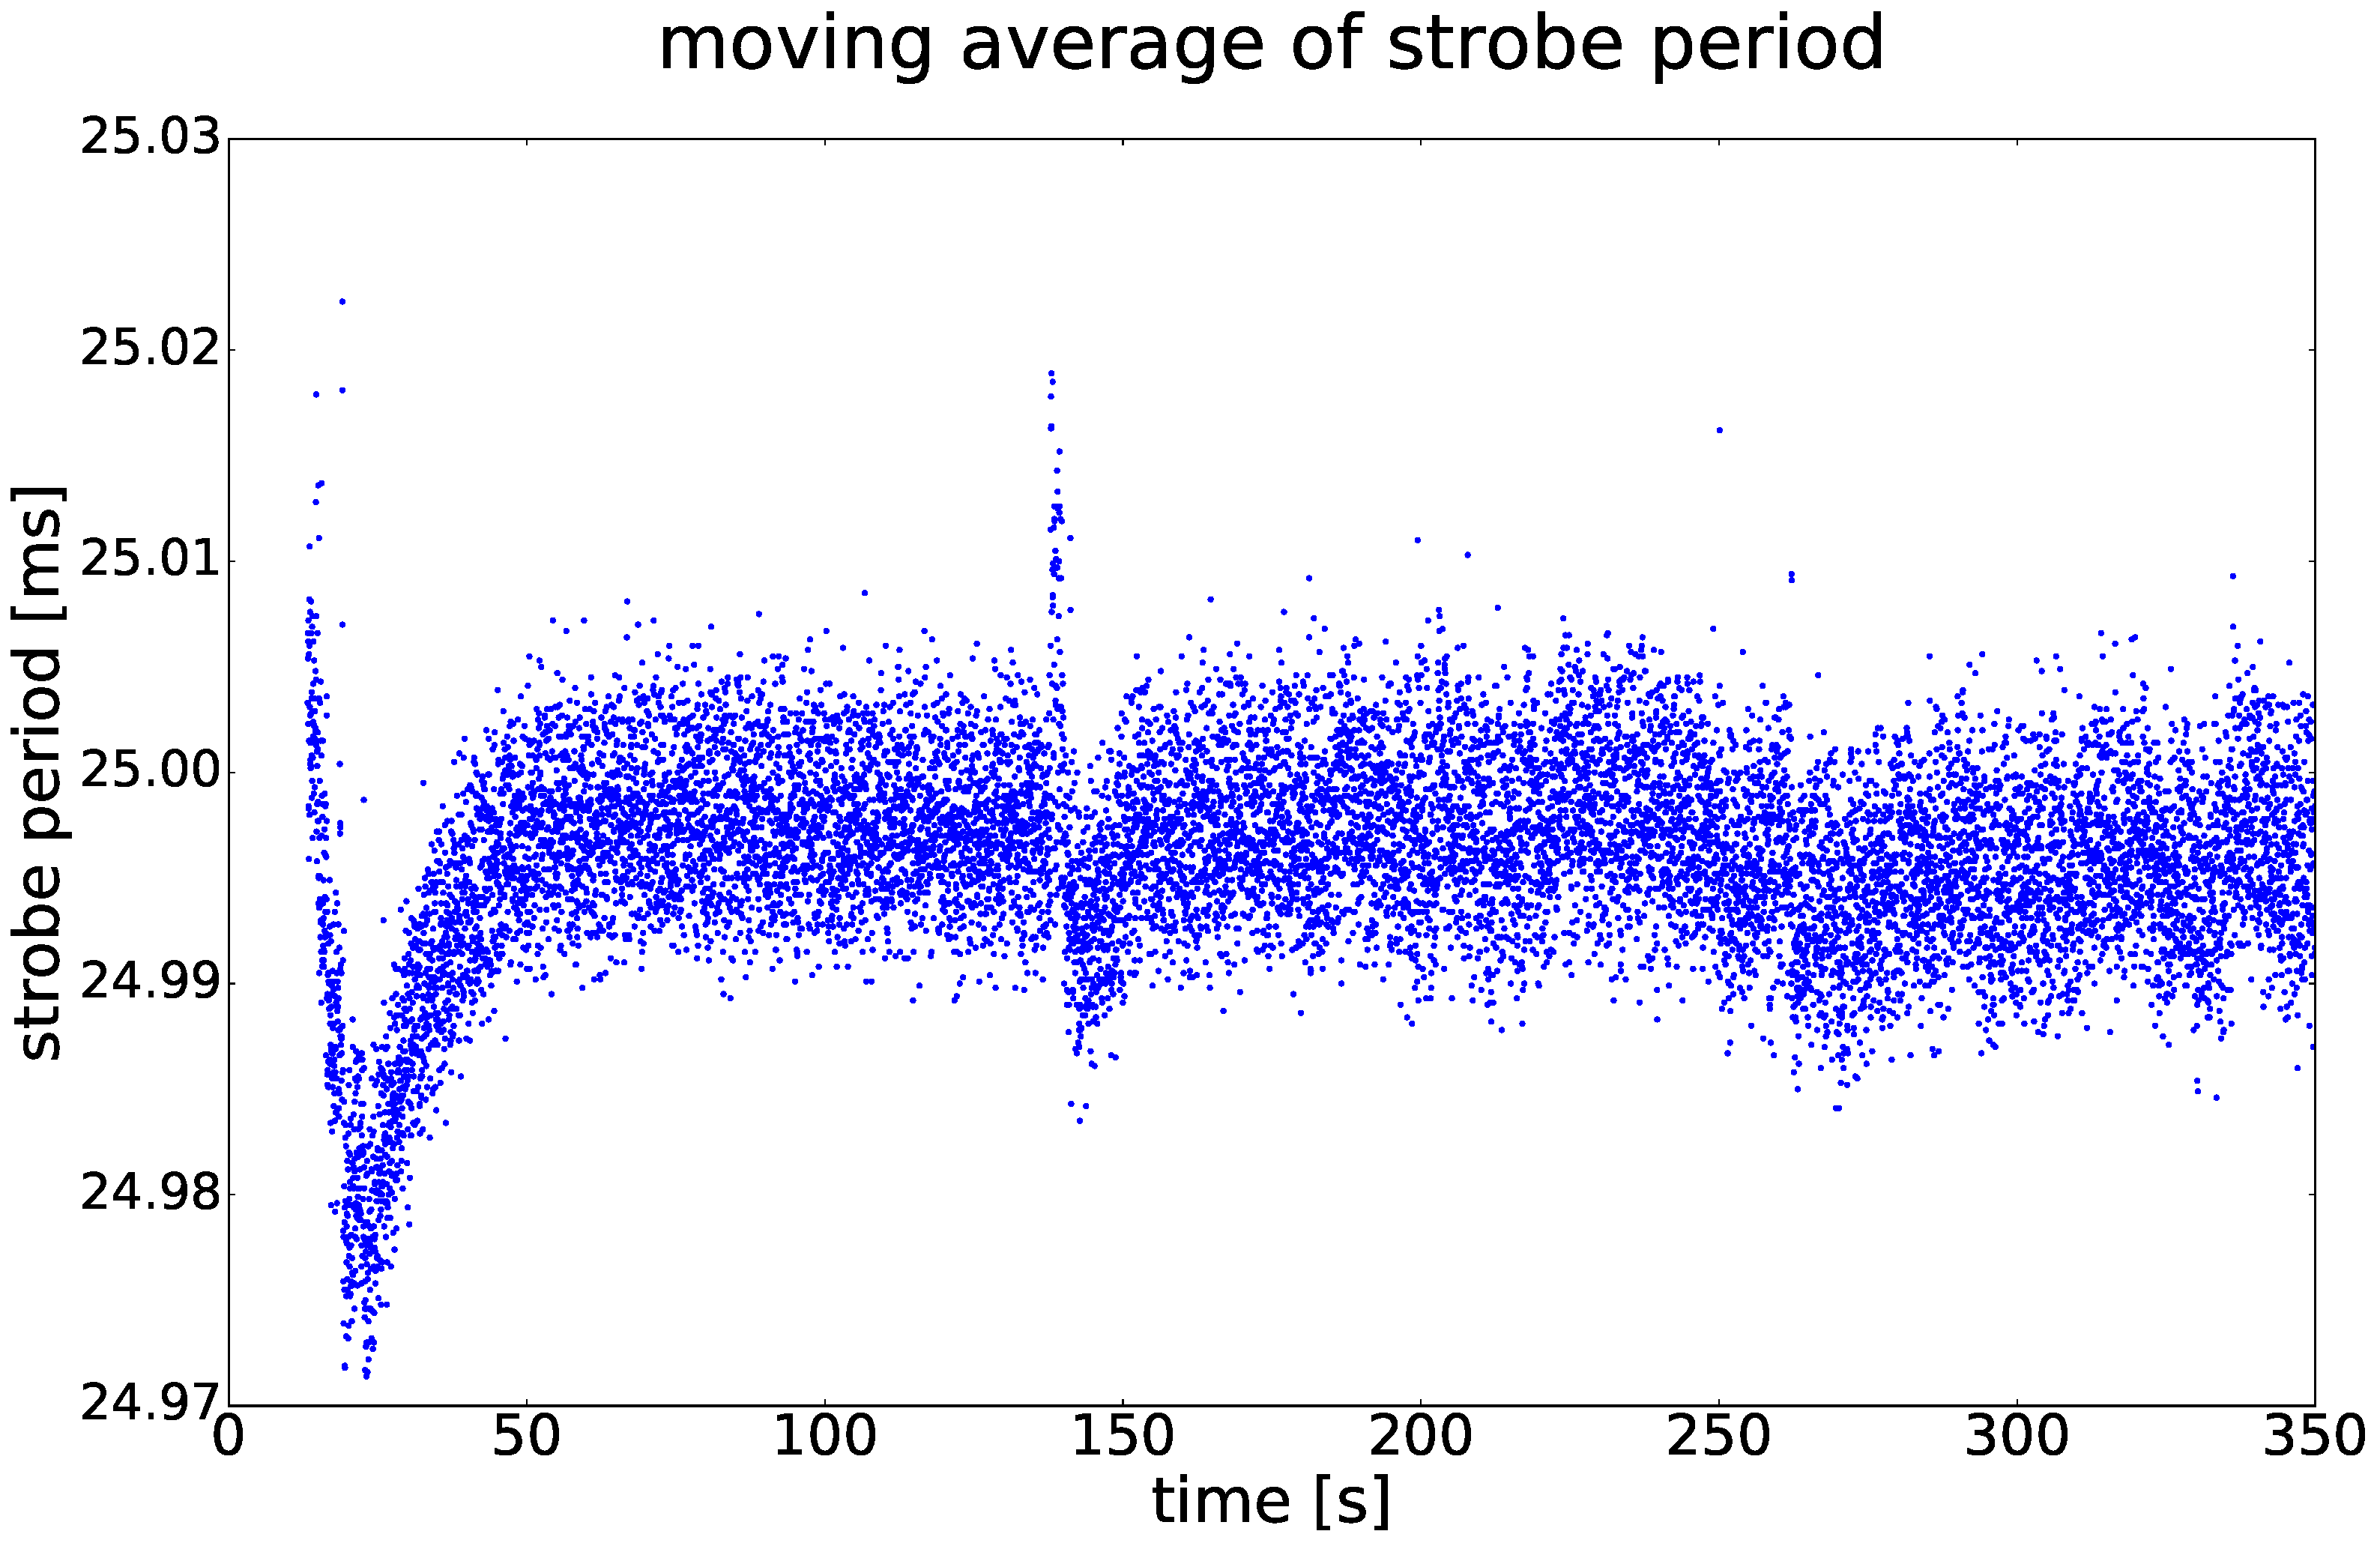
\includegraphics[width=\linewidth]{figures/exp_avg_warmup.pdf}
        \caption{After a short warmup time, the estimated strobe period $\dt$ converges to
          a value of 25ms corresponding to $f=40$Hz. The peak at 140s is
          due to a spike in CPU load caused by a client ROS node
          subscribing to camera images.}
    \label{fig:expavg}
\end{figure}

Due to the scale of the $y$ axis, the strobe period $\dt$ in Fig. \ref{fig:expavg}
seems noisy. However, this must be put into
perspective. Fig. \ref{fig:raw_dt} shows the strobe period $\dtaz$ computed
from raw differences in 
arrival times for camera 0. Compared to the large
noise of the input data, the average (shown in blue) is actually very stable.

\begin{figure}[h]
	\centering
	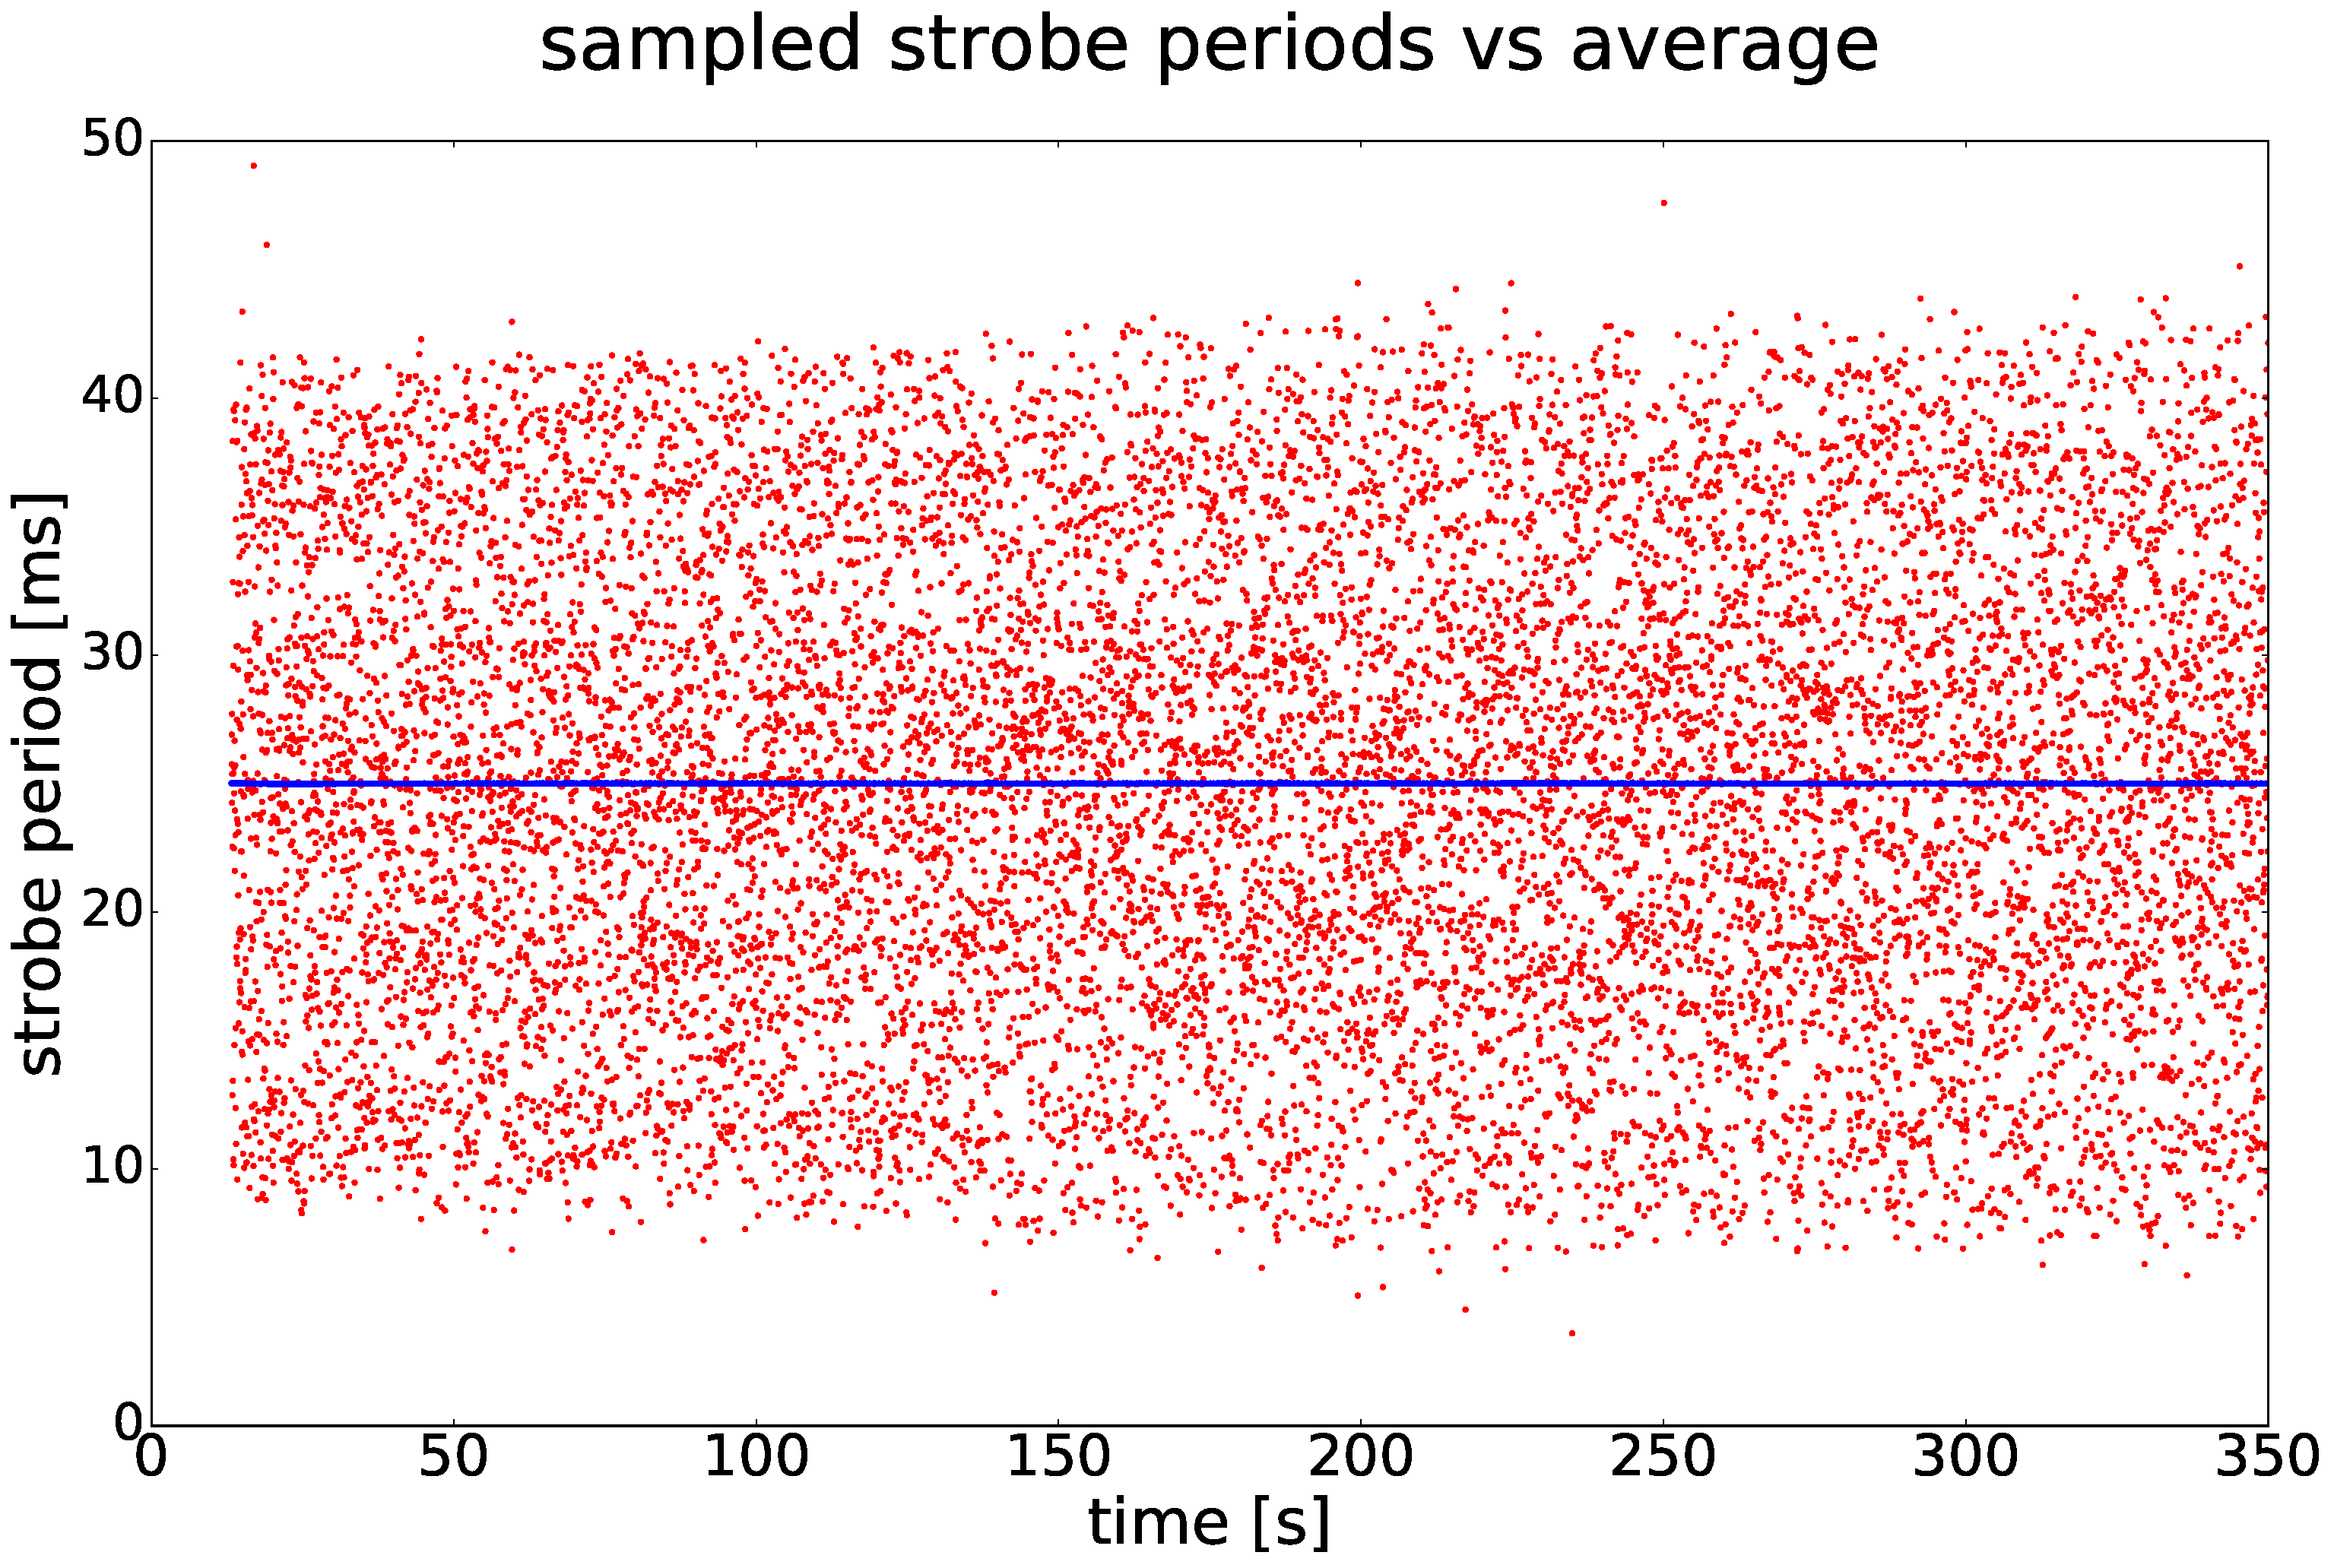
\includegraphics[width=\linewidth]{figures/samples_vs_avg.pdf}
        \caption{Red dots: strobe periods $\dtaz$,
          from camera 0 arrival time differences. Blue dots:
          $\dt$, computed by 10s exponential moving average
          over all camera strobe periods.}
    \label{fig:raw_dt}
\end{figure}

It turns out that $\dt$ is also more stable than differences of
embedded image time stamps. Fig. \ref{fig:embed_dt} shows this cleary.
\begin{figure}[h]
	\centering
	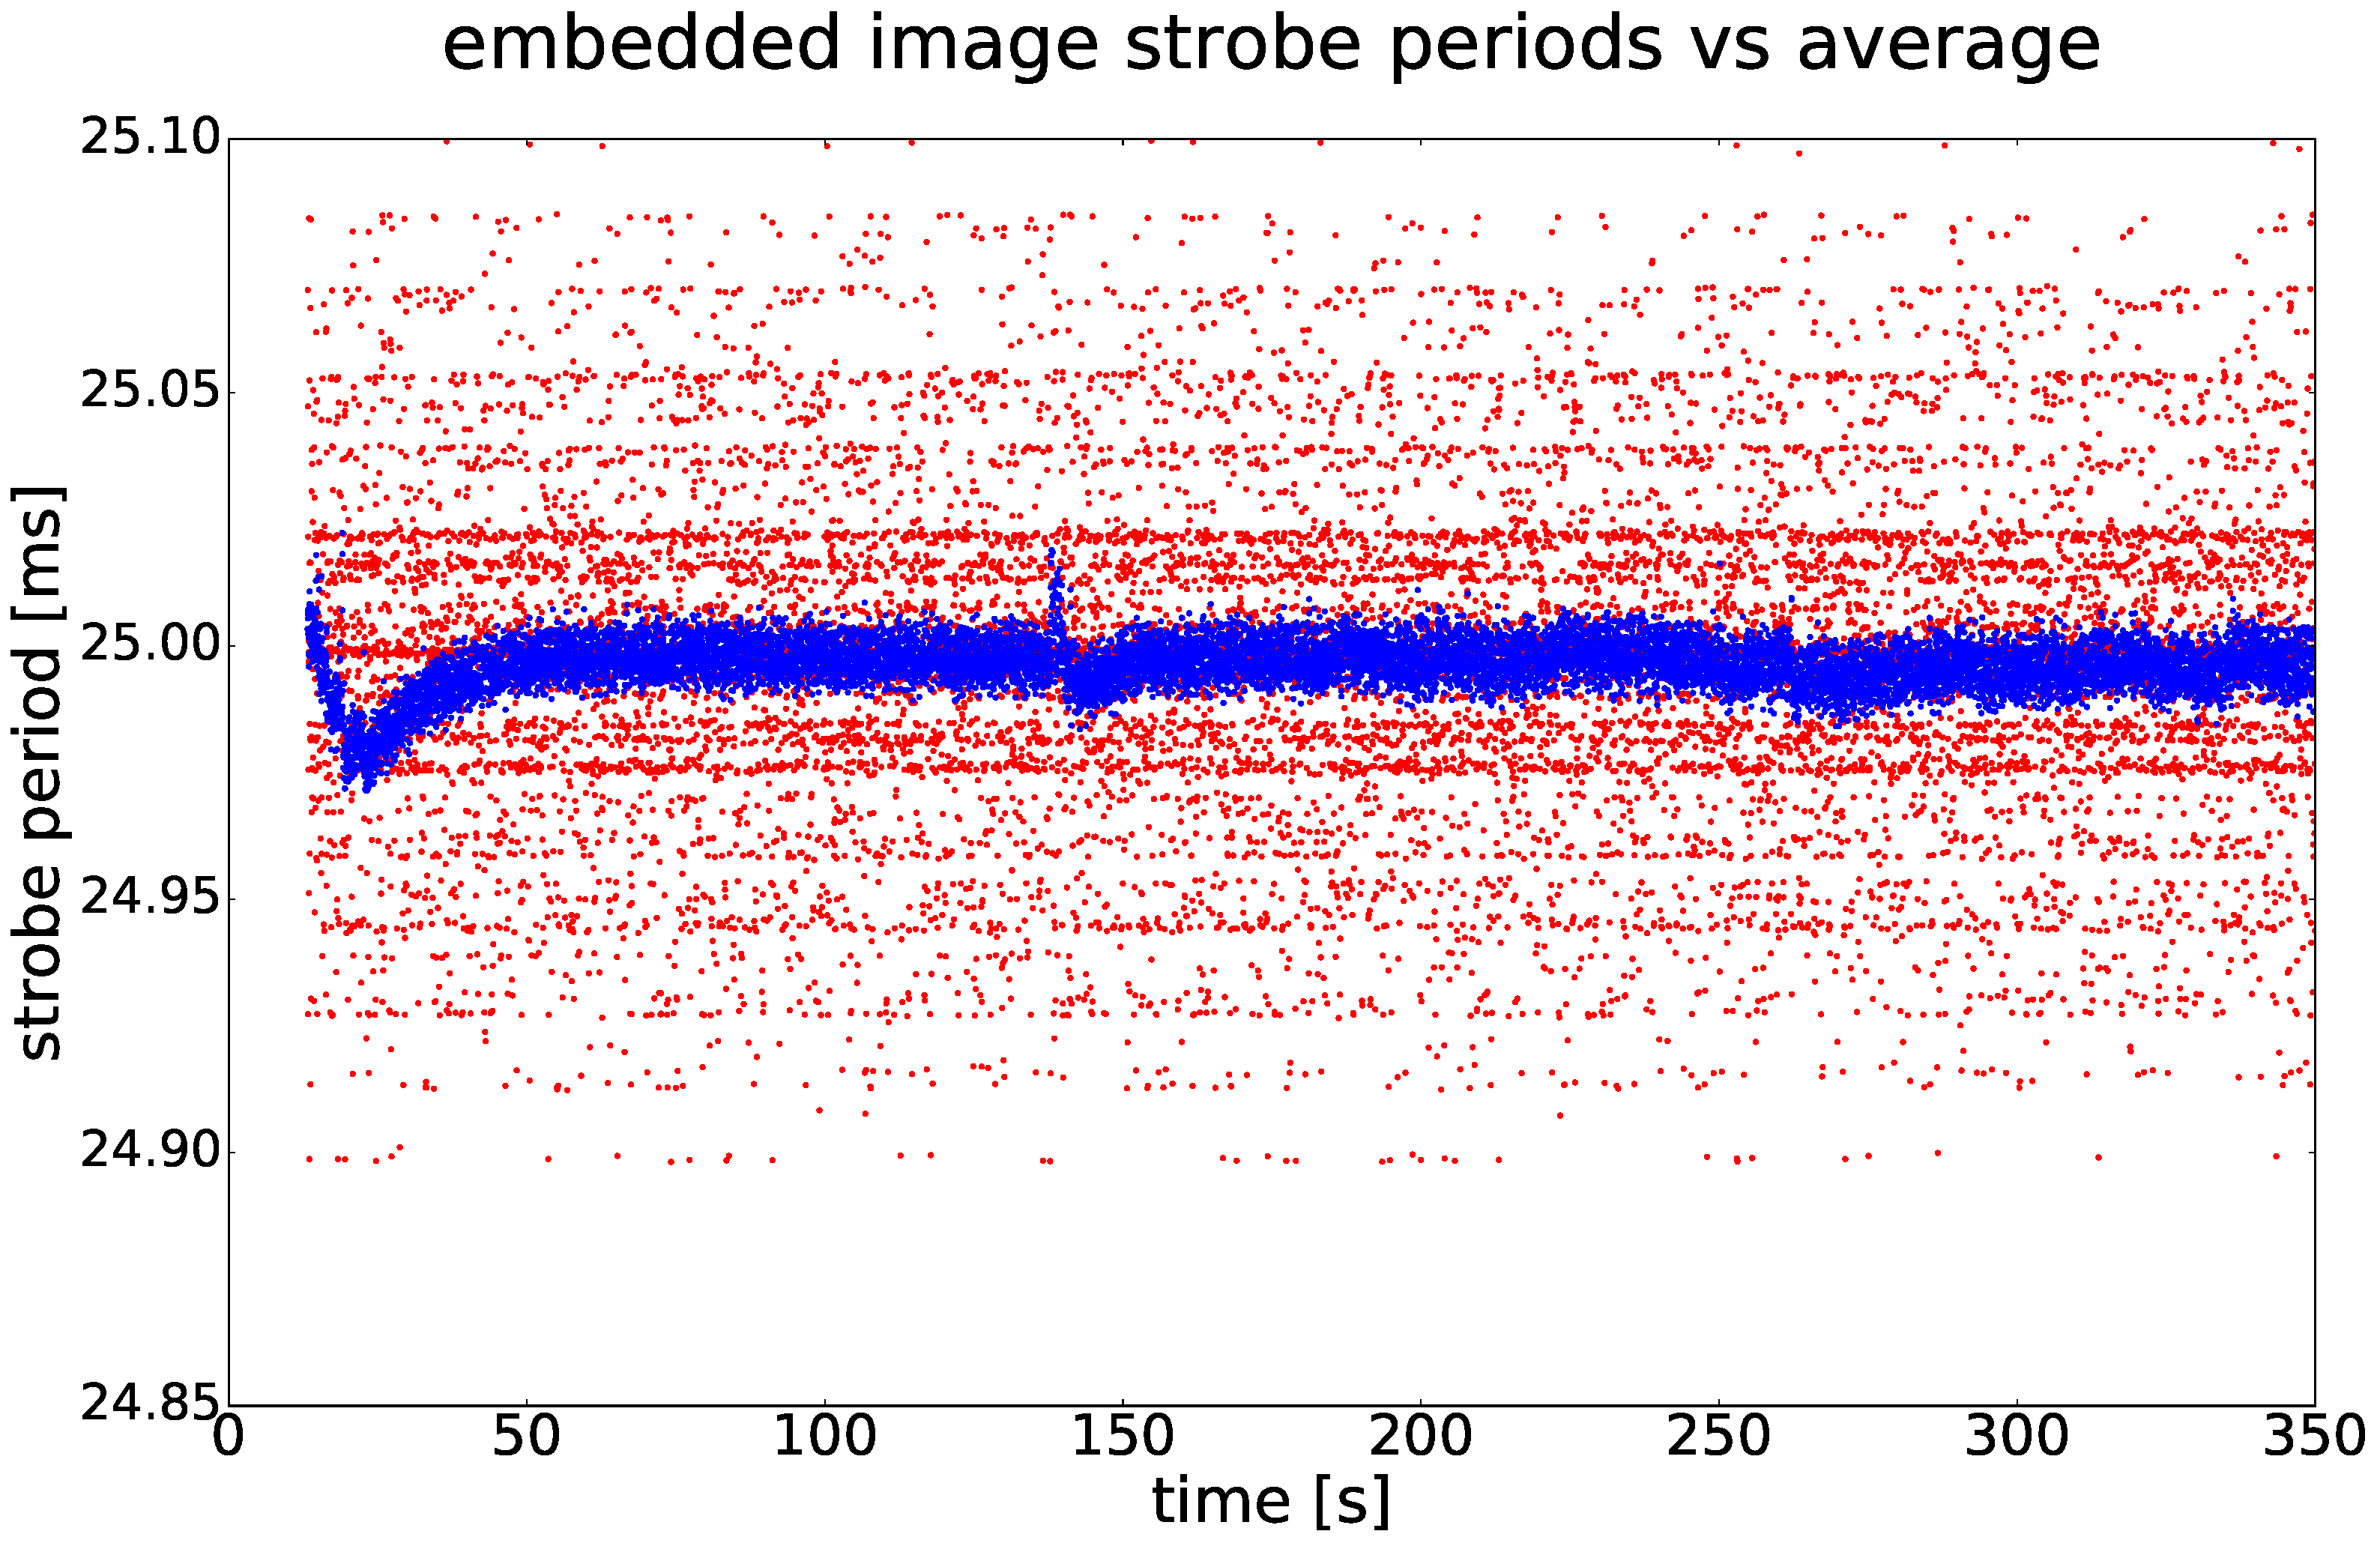
\includegraphics[width=\linewidth]{figures/embedded_vs_avg.pdf}
        \caption{Red dots: strobe periods $\eztime{n}-\eztime{n-1}$,
          computed from embedded image time stamps. Blue dots:
          $\dt$, calculated as moving average over all camera strobe periods.}
    \label{fig:embed_dt}
\end{figure}

After the start of the camera drivers, it takes about 30-50 seconds for
all cameras to produce frames at a reliable frame rate and for frame
drops to become less frequent. To decide when this warm up period has
ended, and  $\dt$ has stabilized, we compute another
moving average, but this time for the relative error from the currently
estimated mean:
\begin{equation}
V_n = V_{n-1} (1 - \alpha) + \alpha \left(\frac{\dtn{n} -
  \dtn{n-1}}{\dtn{n}}\right)^2\ .  
\end{equation}
$V$ measures something similar to the variance of the
updates to the average. When those updates are less than 1\%,
i.e. when $V_n < 0.01^2$, we consider the warm up period complete.


\subsection{Maintaining per-camera estimated pulse time}

Once a stable strobe period $\dt$ is available, one can use it to maintain an
estimate of the camera time for camera $i$:
\begin{equation}
\label{eq:camt}
\ttime{n} = \ttime{n-k} + k\dt + \beta(\atime{n} - (\ttime{n-k} + k\dt))\ ,
\end{equation}
where $k$ is the number of frames that have passed, as computed from Eq. \ref{eq:nframes}.
For the first frame, we set $\ttime{0} = \atime{0}$. The main innovation
to the camera time in Eq. \ref{eq:camt} obviously comes from $k\dt$, but
there is another term which mixes in a small amount ($\beta = 0.005$) of the difference
between the actual arrival time and the predicted camera time, thereby ensuring
that in the long run and on average, the camera time will not
drift away from the arrival time.
By means of Eq. \ref{eq:camt} we associate an arriving frame with the
time at which it was triggered at the camera, even if it arrives late due to temporary network
or CPU load. Due to the large reduction of jitter, the camera time $\ttime{}$ is
suitable for grouping frames by sync pulse, as shown in Fig. \ref{fig:arrival_vs_frame}.


\subsection{Assigning time stamps to frames}
When a frame arrives at the host and produces a new camera time
$\ttime{n}$ according to Eq. \ref{eq:camt}, it must then be associated with
a global time $T_n$ with which all frames belonging to this pulse $n$ are labeled.
For this purpose, a sorted list of times
$T_n$ is maintained, as well as an accumulator $\delta$.
At the start, $\delta$ is initialized to zero and the sorted list of
global times is cleared.

Upon arrival of a new frame, the sorted list is searched based on
$\ttime{n}$ and the following actions are taken:
\begin{itemize}
\item If the camera time of the arriving frame is close to a $T_n$ in
  the list, i.e.  $|T_n - \ttime{n}| \leq  \dt/2$, then
  it is associated with that $T_n$, and $T_n$ is the time stamp under
  which that camera frame will be published. Any difference is
  accumulated: $\delta \leftarrow \delta + (\ttime{n} - T_n)/N$, to be used
  subsequently.
\item If no list element close to $\ttime{n}$ is found, the camera frame
  establishes a new global time: $T_n
  =\ttime{n} + \delta$, which is entered into the sorted list, and $\delta$
  is reset to zero.
\end{itemize}
Without adding $\delta$, the time $T_n$ would be set to the time
$\ttime{n}$ of the first camera $i$ for which a frame arrives.
This would not be an issue if the arrival order of cameras were random.
In practice however we observe
persistent ordering in the arrival of frames. An obvious reason for
this are differences in shutter time, but thread scheduling policies,
interrupt priorities, FLIR driver implementation details, 
and the order in which incoming packets are processed by the network
interfaces could potentially all contribute to persistent
ordering. Adding $\delta$ causes $T_n$ to align with the mean of
the frame arrival times, and so improve the robustness of the
assignment.

\subsection{Monitoring correct association}
Given the large amount of noise in the arrival times of the frames, the
danger of persistently grouping the frames incorrectly, and thereby
generating systematically flawed data is very real. The method
presented in the preceeding subsections is not only robust to such failures, but can
easily produce statistics that directly demonstrate the validity of frame
associations. This can be done by simply computing for each camera $i$
the difference
\begin{equation}
^{(i)}\epsilon_n = (\atime{n} - T_n)/T_n
\end{equation}
between the arrival time of a frame, and the frame time $T_n$ that was
assigned to it. This quantity will obviously be very noisy, since the
frame time $T_n$ has low jitter, whereas $\atime{n}$ is
unfiltered. We therefore compute a moving average again:
\begin{equation}
\label{eq:eavg}
^{(i)}E_n = (1 - \gamma)\ ^{(i)}E_{n-1} + \gamma\ ^{(i)}\epsilon_n\ ,
\end{equation}
with a constant $\gamma = 0.025$ that corresponds to a time horizon of
about one second.

\begin{figure}[h]
	\centering
	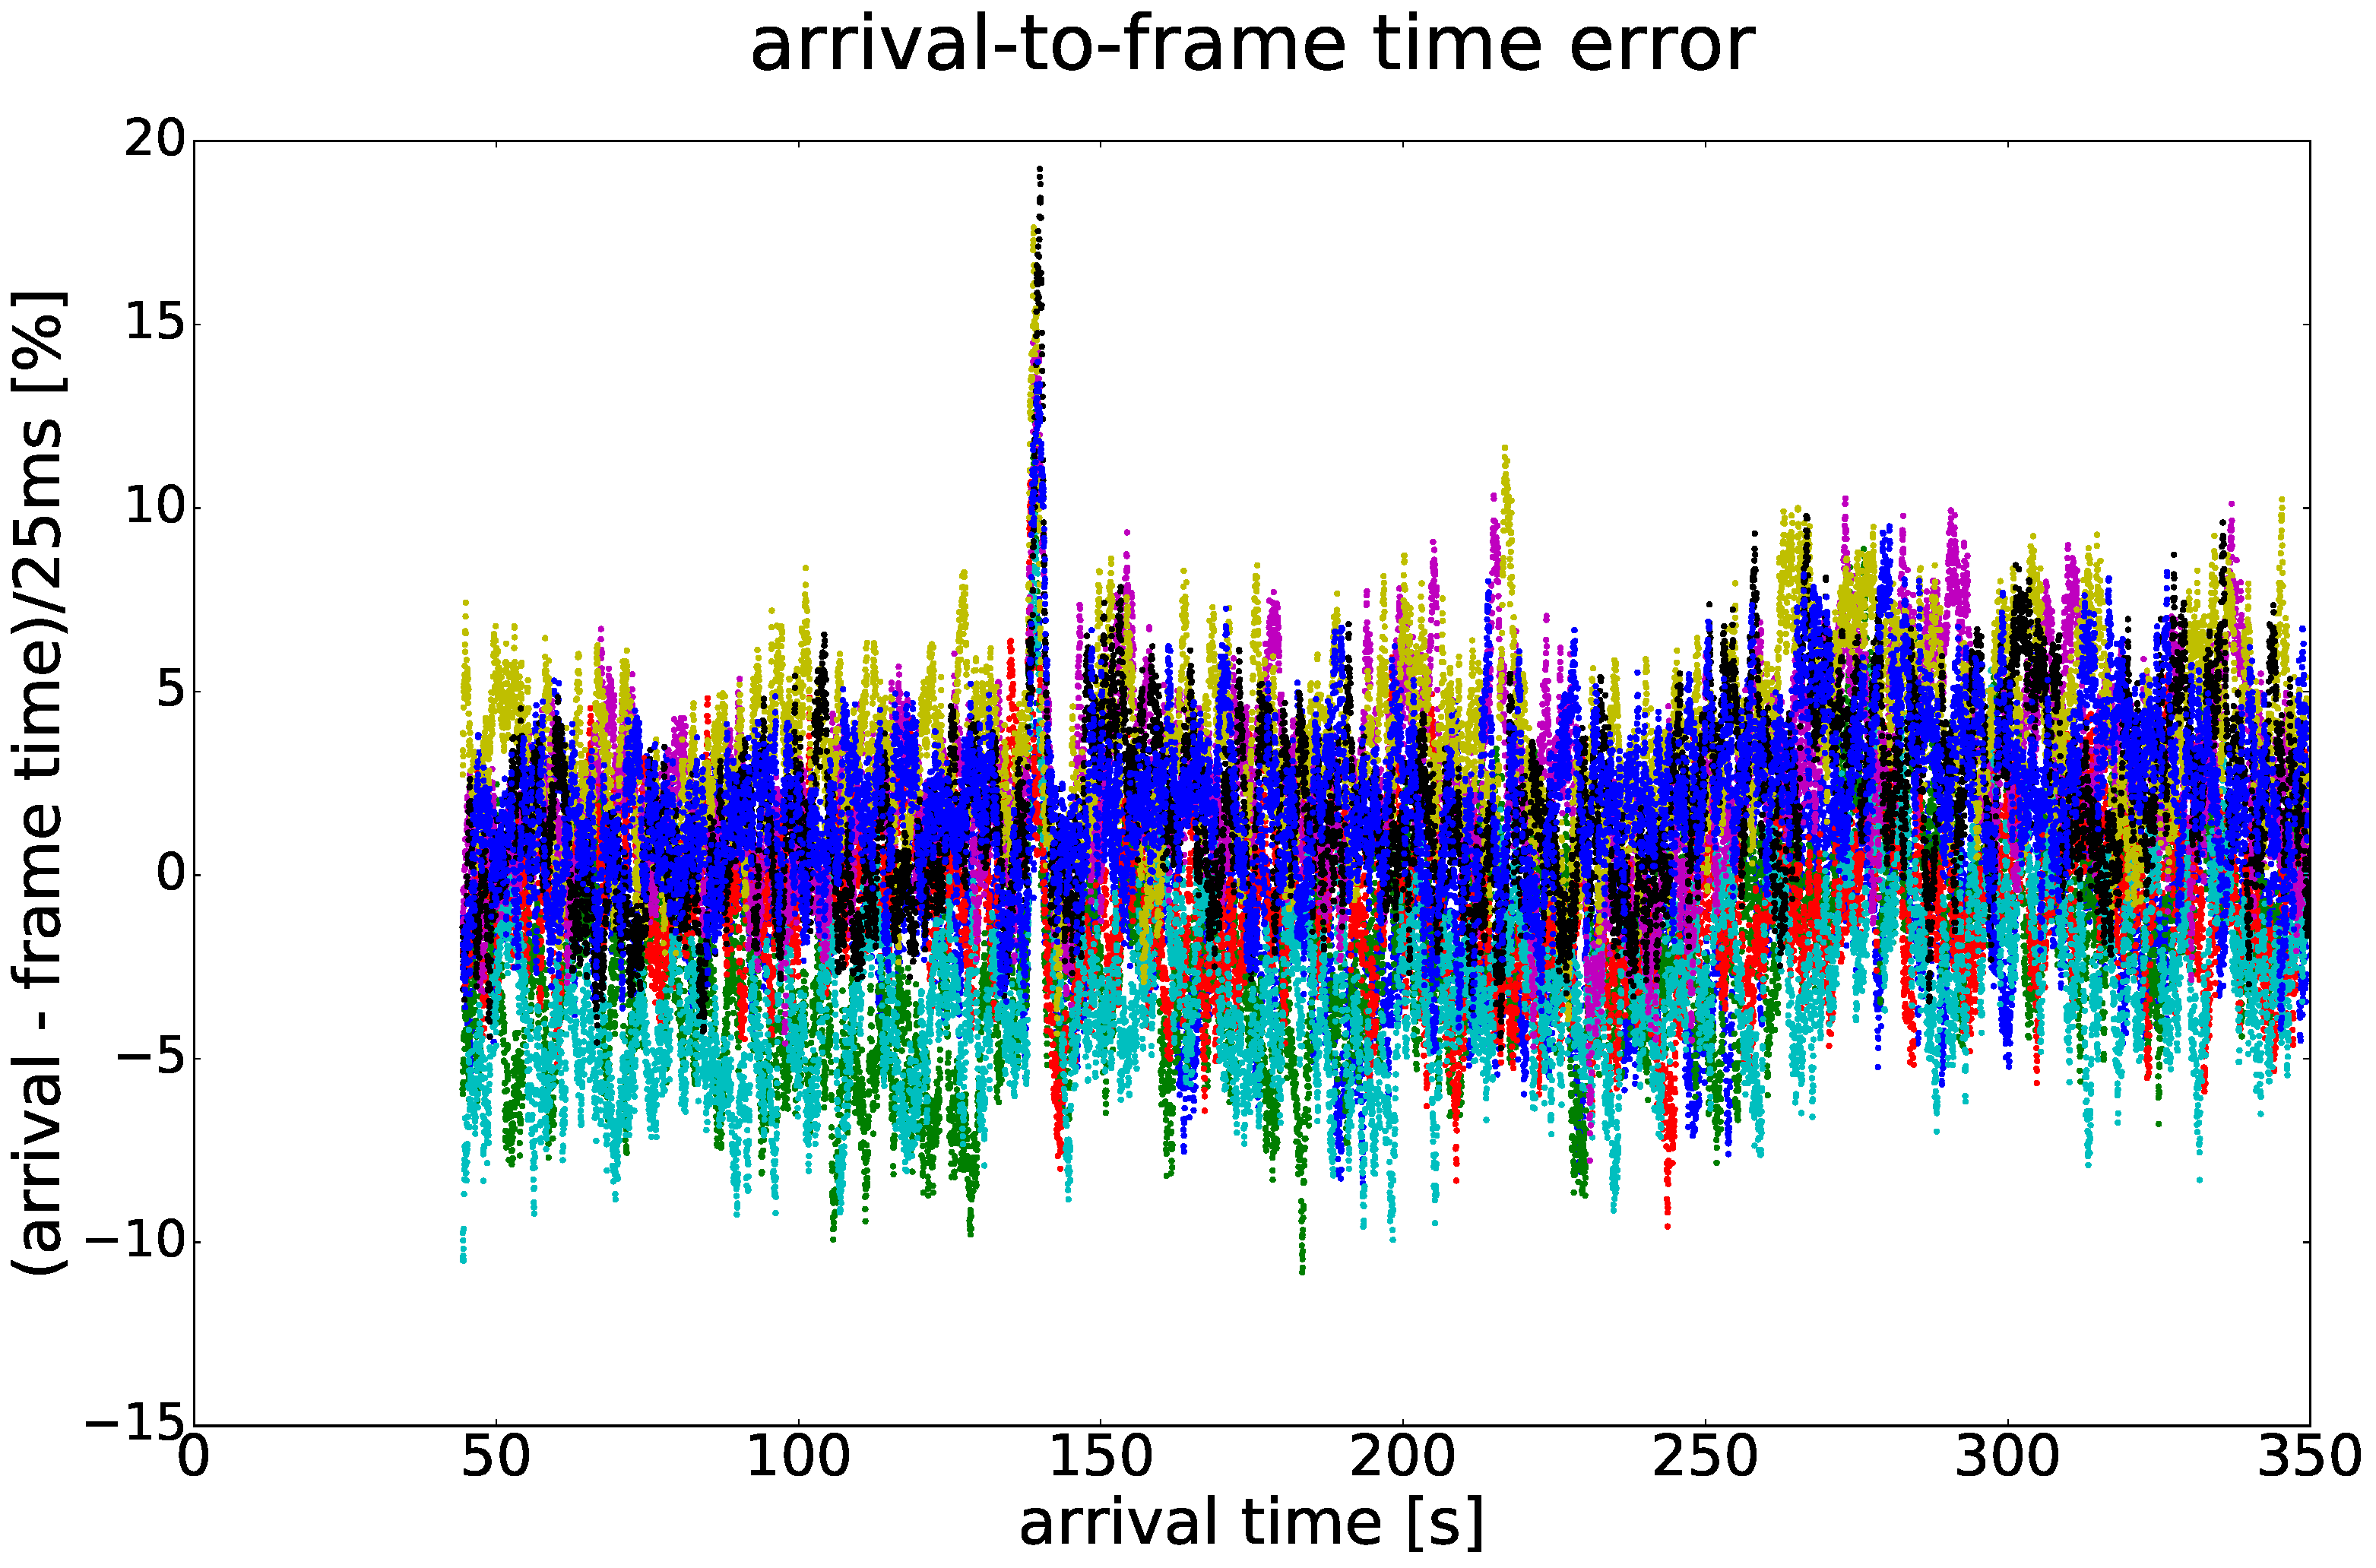
\includegraphics[width=\linewidth]{figures/monitoring.pdf}
        \caption{Plot of monitoring error $E$ (Eq. \ref{eq:eavg}) in
          \% of a full frame period, as a
          function of time for the post warm-up period. Each color
          corresponds to a different camera. Note how $E$ stays below
          20\% even when the load spike occurs at about 140s. One can also
          see that frames from certain cameras arrive consistently
          earlier than from others.}
    \label{fig:monitor}
\end{figure}

As Fig. \ref{fig:monitor} shows, the 1-second averaged error $E$ between
frame arrival time and frame time fluctuates between about -10\% and
+10\% of a full frame period (25ms). When a sudden load is put on the
system, $E$ can spike up to about 20\%, but quickly recovers.

In the actual implementation of CamSync, the averaged error $E$, along
with its standard deviation, are printed out once a minute. Failure to
pass other sanity checks (e.g. the same frame time being assigned to
consecutive frames for the same camera) are reported as well.
